\documentclass[12pt]{article}%
\usepackage{amsfonts}
\usepackage{fancyhdr}
\usepackage{comment}
\usepackage[letterpaper, top=2.5cm, bottom=2.5cm, left=2.2cm, right=2.2cm]%
{geometry}
\usepackage{times}
\usepackage{amsmath}
\usepackage{changepage}
\usepackage{multirow}
\usepackage{amssymb}
\usepackage{tikz}
\usetikzlibrary{arrows.meta}
\usepackage{graphicx}%
\graphicspath{ {images/} }
\usepackage{amsmath}
\setcounter{MaxMatrixCols}{30}
\newtheorem{theorem}{Theorem}
\newtheorem{acknowledgement}[theorem]{Acknowledgement}
\newtheorem{algorithm}[theorem]{Algorithm}
\newtheorem{axiom}{Axiom}
\newtheorem{case}[theorem]{Case}
\newtheorem{claim}[theorem]{Claim}
\newtheorem{conclusion}[theorem]{Conclusion}
\newtheorem{condition}[theorem]{Condition}
\newtheorem{conjecture}[theorem]{Conjecture}
\newtheorem{corollary}[theorem]{Corollary}
\newtheorem{criterion}[theorem]{Criterion}
\newtheorem{definition}[theorem]{Definition}
\newtheorem{example}[theorem]{Example}
\newtheorem{exercise}[theorem]{Exercise}
\newtheorem{lemma}[theorem]{Lemma}
\newtheorem{notation}[theorem]{Notation}
\newtheorem{problem}[theorem]{Problem}
\newtheorem{proposition}[theorem]{Proposition}
\newtheorem{remark}[theorem]{Remark}
\newtheorem{solution}[theorem]{Solution}
\newtheorem{summary}[theorem]{Summary}
\newenvironment{proof}[1][Proof]{\textbf{#1.} }{\ \rule{0.5em}{0.5em}}

\newcommand{\Q}{\mathbb{Q}}
\newcommand{\R}{\mathbb{R}}
\newcommand{\C}{\mathbb{C}}
\newcommand{\Z}{\mathbb{Z}}

\newcommand*{\pd}[3][]{\ensuremath{\frac{\partial^{#1} #2}{\partial #3}}}

\usepackage{enumerate}% http://ctan.org/pkg/enumerate
\usepackage{array}% http://ctan.org/pkg/array
\newcolumntype{M}{>{$}c<{$}}


\begin{document}

\title{CS 440/ECE448 Homework 5}
\author{Tanishq Dubey (tdubey3)}
\date{\today}
\maketitle
\section*{Problem 1}
    \begin{enumerate}[a)]
        \item
            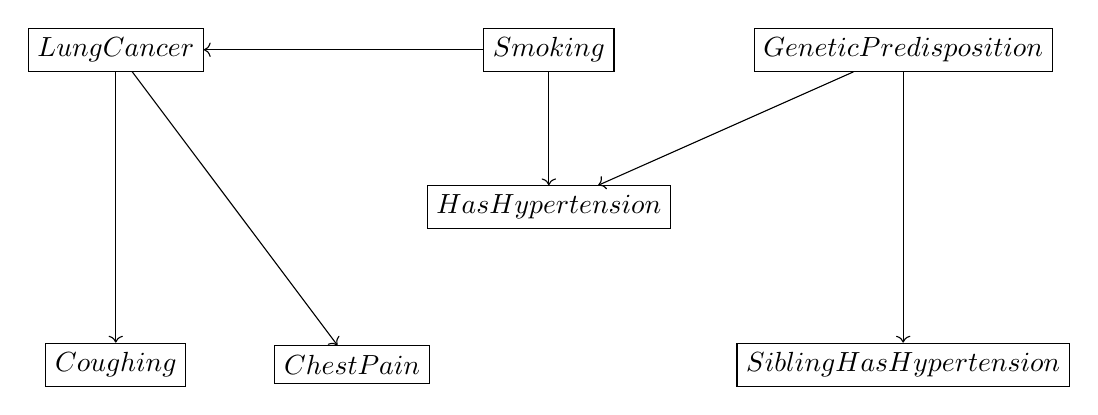
\begin{tikzpicture}
                \node[shape=rectangle,draw=black] (A) at (5.5,0) {$HasHypertension$};
                \node[shape=rectangle,draw=black] (B) at (5.5,2) {$Smoking$};
                \node[shape=rectangle,draw=black] (C) at (10,2) {$GeneticPredisposition$};
                \node[shape=rectangle,draw=black] (D) at (0, 2) {$LungCancer$};
                \node[shape=rectangle,draw=black] (E) at (10,-2) {$SiblingHasHypertension$};
                \node[shape=rectangle,draw=black] (F) at (0, -2) {$Coughing$} ;
                \node[shape=rectangle,draw=black] (G) at (3, -2) {$ChestPain$} ;
            
                \path [->](B) edge node[left] {} (A);
                \path [->](C) edge node[left] {} (A);
                \path [->](B) edge node[left] {} (D);
                \path [->](D) edge node[left] {} (F);
                \path [->](D) edge node[right] {} (G);
                \path [->](C) edge node[right] {} (E);
            \end{tikzpicture}
        \item
            $14$ parameters are the minimum needed to encode this Bayes net.
        \item
            $2^7-1$ parameters are needed for the full joint probability distribution.
        \item
            New phone, who dis.
    \end{enumerate}

\section*{Problem 2}
    \begin{enumerate}[a)]
        \item The values $a$ through $h$ are as follows:
            \[a=.3\]
            \[b=.6\]
            \[c=.3\]
            \[d=.5\]
            \[e=.4\]
            \[f=.7\]
            \[g=.5\]
            \[h=.4\]
        \newpage
        \item
            \begin{align*}
                \textbf{P}(D=T | A=F) = \textbf{P}(D=T|C=T)\textbf{P}(C=T|A=F,B=T)\textbf{P}(B=T)\\
                +\textbf{P}(D=T|C=T)\textbf{P}(C=T|A=F,B=F)\textbf{P}(B=F)\\
                +\textbf{P}(D=T|C=F)\textbf{P}(C=F|A=F,B=T)\textbf{P}(B=T)\\
                +\textbf{P}(D=T|C=F)\textbf{P}(C=F|A=F,B=F)\textbf{P}(B=F)\\
            \end{align*}
            This then leads to:
            \[\textbf{P}(D=T|A=F)= geb+gf(1-b)+h(1-e)b+h(1-f)(1-b)\]
        \item
            \[\textbf{P}(B = F | A = T) = \textbf{P}(B = F)\]
            This then leads to:
            \[\textbf{P}(B = F | A = T) = 1-b\]
        \item
            From Part B:
            \[\textbf{P}(D=T|A=F) = geb+gf(1-b)+h(1-e)b+h(1-f)(1-b)\]
            The values found in part A can be substituted in:
            \[\textbf{P}(D=T|A=F) = (0.5)(0.4)(0.6)+(0.5)(0.7)(0.4)+(0.4)(0.6)(0.6)+(0.4)(0.4)(0.4)\]
            Thusly:
            \[\textbf{P}(D=T|A=F) = 0.452\]
    \end{enumerate}
\section*{Problem 3}
    \begin{enumerate}[a)]
        \item
            The number of parameters need to represent the full joint for all 6 Bayes nets is:
            \[N_AN_BN_CN_DN_EN_F - 1\]
        \item
            The minimum number of parameters needed for to represent each of the 6 Bayes nets is as follows:
            \begin{enumerate}[(1)]
                \item
                    \[(N_A -1) + N_A(N_C -1) + N_C(N_E -1) + (N_B -1) + N_B(N_D -1) + N_D(N_F - 1)\]
                \item
                    \[(N_A -1) + N_A(N_C -1) + N_C(N_E -1) + (N_B -1) + N_B(N_D -1) + N_CN_D(N_F - 1)\]
                \item
                    \[(N_A -1) + N_A(N_C -1) + N_C(N_E -1) + (N_B -1) + N_AN_B(N_D -1) + N_D(N_F - 1)\]
                \item
                    \[(N_A -1) + N_A(N_C -1) + N_C(N_E -1) + (N_B -1) + N_AN_B(N_D -1) + N_CN_D(N_F - 1)\]
                \item
                    \[(N_A -1) + N_BN_A(N_C -1) + N_C(N_E -1) + (N_B -1) + N_AN_B(N_D -1) + N_D(N_F - 1)\]
                \item
                    \[(N_A -1) + N_BN_A(N_C -1) + N_C(N_E -1) + (N_B -1) + N_AN_B(N_D -1) + N_CN_D(N_F - 1)\]
            \end{enumerate}
    \end{enumerate}
\end{document}